\begin{figure}[h!]
    \centering
    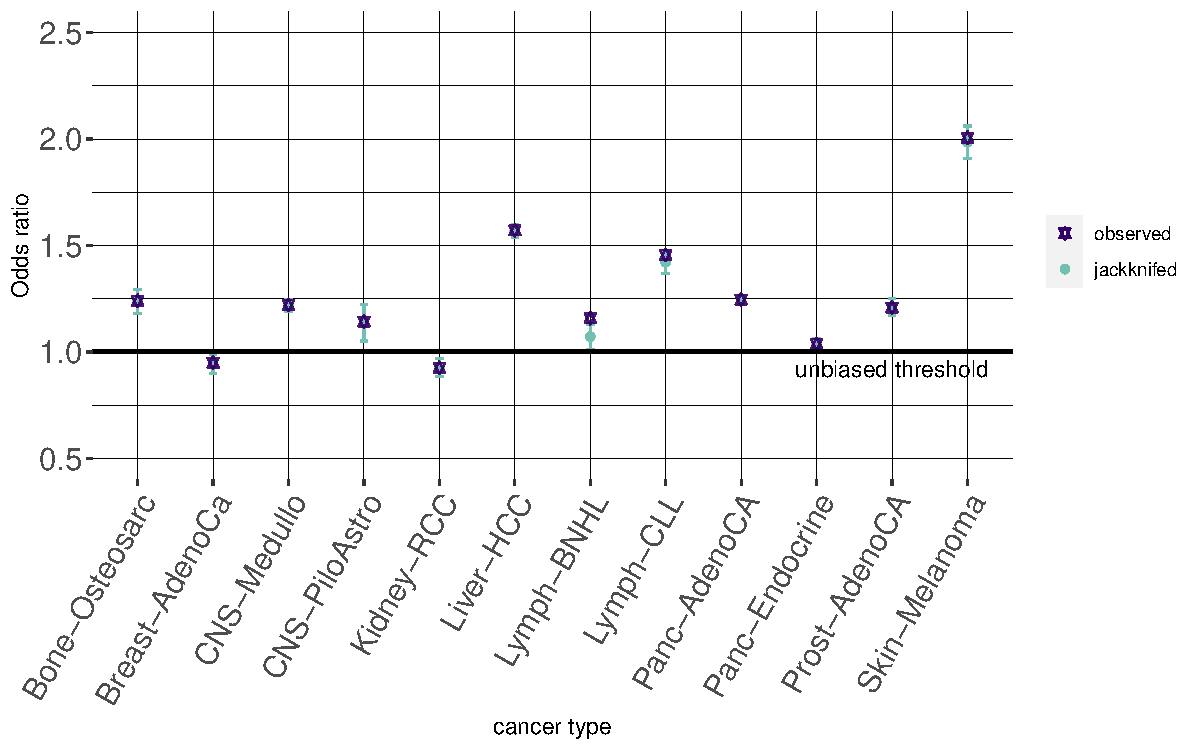
\includegraphics[scale=0.8]{graphics/jackknife_OR.pdf}
    \caption{\textbf{Mutations tend to occur in closed chromatin regions according to the odds ratio ($OR$) statistic}. $OR>1$ indicates a bias towards towards closed regions, and $OR<1$ indicates the opposite. Error bars are the standard errors of the jackknifed sample. The green points are the means of the jackknifed pseudo-values. The purple points are the observed $OR$.}
    \label{fig:or_jackknifed}
\end{figure}
